\renewcommand{\theequation}{1.\arabic{equation}}
\begin{enumerate}[label=(\alph*)]

\item 

\textbf{Hệ quy chiếu gắn với cây:}

Dựa vào các điều kiện ban đầu, ta thiết lập các phương trình chuyển động của ba vật, lần lượt của
\begin{itemize}
  \item Cây: \begin{equation}
    x_{C}(t)=0.
  \end{equation}
  \item Xe: \begin{equation}
    x_{Xe}(t)=10t.
  \end{equation}
  \item Bóng: \begin{equation}
    x_{B}(t)=10+5t.
  \end{equation}
\end{itemize}
Đây cũng chính là các phương trình của đường thế giới của các vật trên đồ thị $(x,t)$; ta vẽ được đồ thị của chúng như sau:
\begin{figure}[H]
  \centering
  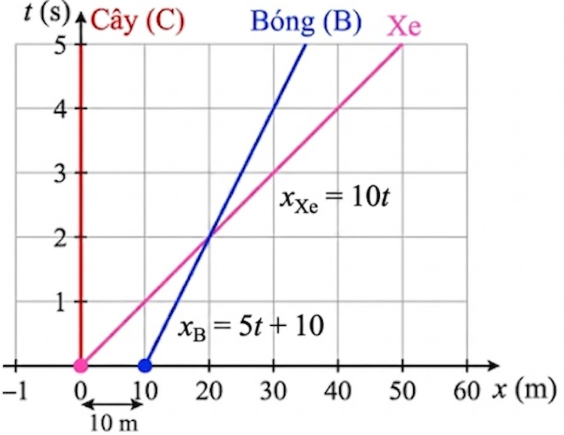
\includegraphics[width=0.5\textwidth]{Problem_1/Image/P1_1.png}
  \caption{Giản đồ không-thời gian trong hệ quy chiếu gắn với cây}
  \label{P1_1}
\end{figure}

\textbf{Hệ quy chiếu gắn với xe:}

Ta chọn chiều dương trục Ox' sao cho tại $t=0$, quả bóng nằm ở phía trục dương. Vận tốc của quả bóng được đo trong hệ quy chiếu của xe là
\begin{equation}
  v_{B}'=v_B-v_{Xe}=-5 \text{ (m/s)}.
\end{equation}
Phương trình đường thế giới của bóng trong hệ quy chiếu của xe do đó là
\begin{equation}
  x_{B}'(t')=10-5t'.
\end{equation}
Vận tốc của cây so với xe:
\begin{equation}
  v_{C}'=0-v_{Xe} =-10 \text{ (m/s)}.
\end{equation}
Phương trình đường thế giới của cây lúc này trở thành
\begin{equation}
  x_{C}'(t')=-10t'.
\end{equation}
Dựa vào đó ta vẽ được:
\begin{figure}[H]
  \centering
  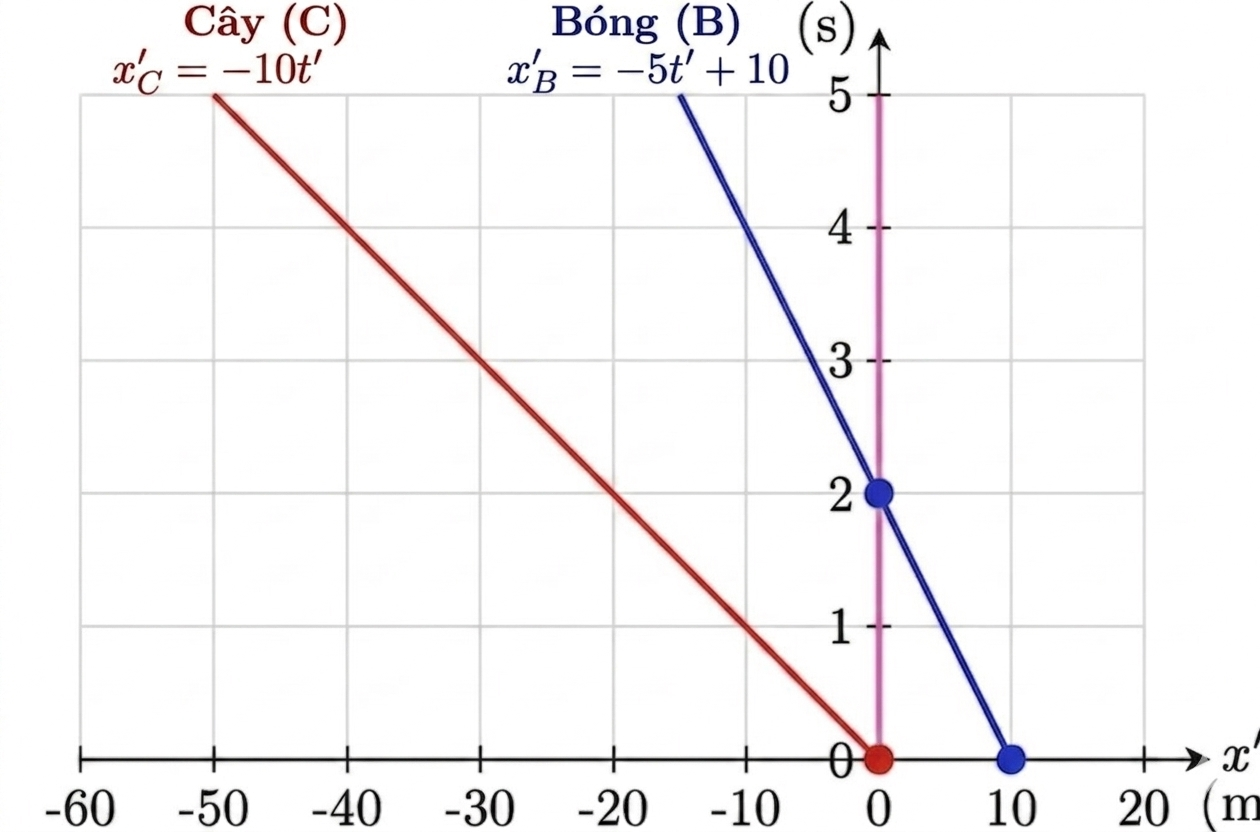
\includegraphics[width=0.5\textwidth]{Problem_1/Image/P1_2.png}
  \caption{Giản đồ không-thời gian trong hệ quy chiếu gắn với xe}
  \label{P1_2}
\end{figure}
\item
Để vẽ được hệ lưới của cây trên giản đồ của xe, ta cần trước tiên xác định các đường đồng thời gian và các đường đồng vị trí trong hệ quy chiếu của cây trên giản đồ của xe.\newline
Các đường đồng vị trí trong hệ quy chiếu của cây miêu tả chuyển động của của những điểm không chuyển động trong hệ quy chiếu này, tức phương trình miêu tả chúng có dạng $x(t)=const$, hay chính là $x'(t)=-10t'+const$; đây là họ các đường song song với đường thế giới của cây trong hệ quy chiếu của xe. Các đường đồng thời gian mô tả các đường nằm ngang thoả mãn $t=const$, mà do ta chấp nhận $t=t'$, chúng cũng thoả mãn $t'=const$, và do đó đơn giản cũng là các đường nằm ngang trên giản đồ của xe. Từ các thông tin trên, ta vẽ được giản đồ sau
\begin{figure}[H]
  \centering
  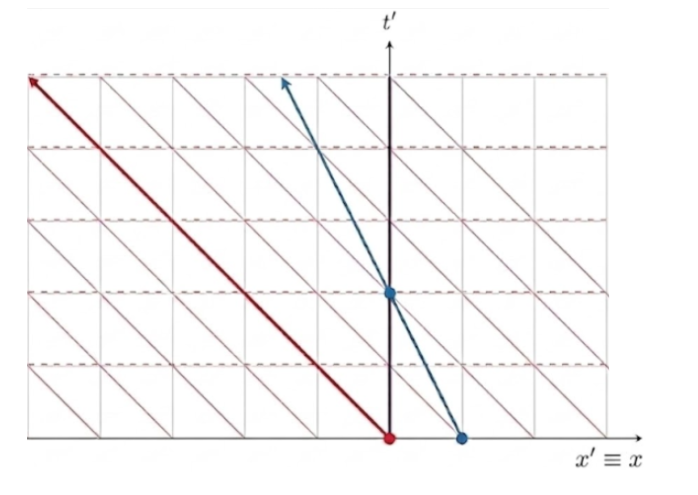
\includegraphics[width=0.5\textwidth]{Problem_1/Image/P1_3.png}
  \caption{Hệ lưới của cây trong giản đồ của xe}
  \label{P1_3}
\end{figure}

Xét một điểm $M$ nào đó có toạ độ $(x',t')$ trên giản đồ của xe (xem \figref{P1_4}): qua $M$, ta kẻ một đường song song với đường thế giới của cây, đường đó cắt trục $Ox$ tại chính xác điểm có toạ độ $x_M$ cần tìm; ta cũng dễ dàng xác định $t_M$. Như vậy phép chiếu lúc này không còn là hạ vuông góc xuống mà là chiếu theo các đường đồng vị trí và đồng thời gian đi qua điểm $M$. Lí do cho thao tác này là vì đường đồng vị trí trong hệ quy chiếu của cây đi qua điểm $M$ là đường thế giới của điểm có toạ độ $x$ không đổi. Ở đây ta đã đặt $M$ lên trên một điểm lưới có sẵn nên không cần phải vẽ thêm nữa.
\begin{figure}[H]
  \centering
  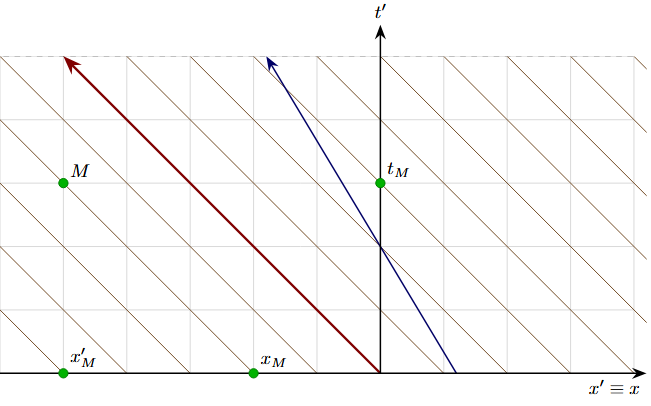
\includegraphics[width=0.5\textwidth]{Problem_1/Image/P1_4.png}
  \caption{Toạ độ điểm M}
  \label{P1_4}
  
\end{figure}  

\vspace{8pt}

\item 
Ta hiểu thế nào là hai sự kiện xảy ra đồng thời trong một hệ quy chiếu? Lấy hai chớp sáng đi ra từ hai điểm $A$ và $B$ như trên giản đồ không-thời gian dưới đây. Trong hệ quy chiếu của cây, chúng tới điểm $C$ tại cùng thời điểm. Vì chúng có cùng tốc độ $c$, đi qua cùng một khoảng cách tới cây, quan sát viên đứng dưới cây sẽ kết luận rằng hai sự kiện tại $A$ và $B$ xảy ra đồng thời. \newline
Mặt khác, chớp sáng từ $B$ chạm tới xe tại điểm $D$, trong khi chớp sáng từ $A$ chạm tới xe tại điểm $E$. Người lái xe sẽ thấy chớp sáng tại $B$ trước $A$. Mà vì chúng trải qua cùng một khoảng cách trong hệ quy chiếu xe với cùng tốc độ $c$, người lái xe sẽ kết luận chớp sáng tại $B$ xảy ra trước $A$.
\begin{figure}[H]
  \centering
  \includegraphics[width=0.6\textwidth]{Problem_1/Image/P1_5.png}
  \caption{}
  \label{P1_5}
\end{figure}
Rõ ràng hai sự kiện xảy ra đồng thời trong hệ quy chiếu này đã không xảy ra đồng thời trong hệ quy chiếu khác. Tổng quát hoá, thời điểm xảy ra của một sự kiện trong hệ quy chiếu này không còn luôn bằng thời điểm xảy ra của nó trong hệ quy chiếu khác.\newline
Ta quay trở lại bài toán được minh họa trong \figref{P1_I3}. 
\begin{figure}[H]
  \centering
  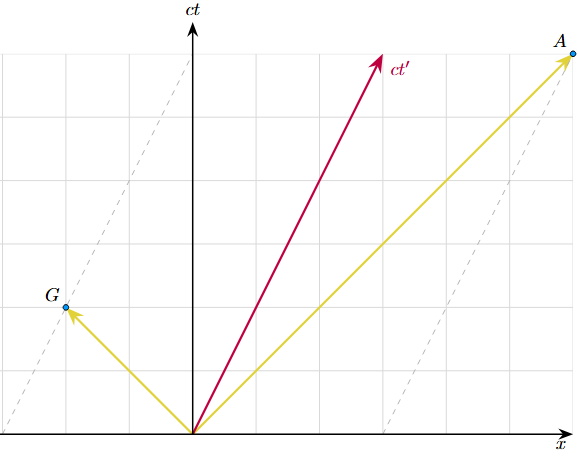
\includegraphics[width=0.5\textwidth]{Problem_1/Image/P1_6.png}
  \caption{}
  \label{P1_6}
\end{figure}
Lấy $A$ và $G$ là hai điểm thuộc đường thế giới của hai điểm không chuyển động trong hệ quy chiếu của xe (hai đường đồng vị trí) mà lại cách đều xe tại thời điểm ban đầu (như trong \figref{P1_6}), có nhận xét rằng khi hai photon tới $A$ và $G$, chúng có cùng khoảng cách tới xe. Trong khi đó, vì tốc độ của hai chớp sáng này đều là $c$ trong hệ quy chiếu của xe, lại xuất phát cùng thời điểm, thời điểm chớp sáng bên trái tới $G$ và thời điểm chớp sáng bên phải tới $A$ trong hệ quy chiếu của xe phải là một. Nghĩa là, $t_{A}'=t_{G}'$.\newline
Đường $AG$ giao với đường thế giới của xe tại $D$. Từ \figref{P1_7}, ta thấy rằng hai chớp sáng xuất phát tại $x_{F}'=x_{G}'$ và $x_{E}'=x_{A}'$ đã tới $D$, tức là vị trí của xe, đồng thời, chúng phải được phát ra đồng thời, hơn nữa, khoảng thời gian trôi qua giữa $E$ và $A$ phải bằng khoảng thời gian trôi qua giữa $F$ và $E$ (khoảng thời giữa giữa thời điểm chúng cùng phát ra chớp sáng và thời điểm chúng cùng nhận chớp sáng ), tất yếu rằng thời điểm hai chớp sáng đi ra từ $O$ để tới $A$, $G$ chính là thời điểm hai chớp sáng đi ra từ $E$, $F$ để tới $D$. Nói cách khác, $t_{E}'=t_{F}'=t_{O}'=0$. Và kéo theo đó là $t_{D}'=t_{A}'=t_{G}'.$
\begin{figure}[H]
  \centering
  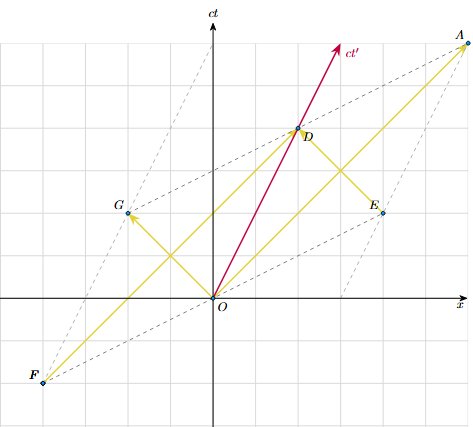
\includegraphics[width=0.5\textwidth]{Problem_1/Image/P1_7.png}
  \caption{}
  \label{P1_7}
  
\end{figure}
\begin{figure}[H]
  \centering
  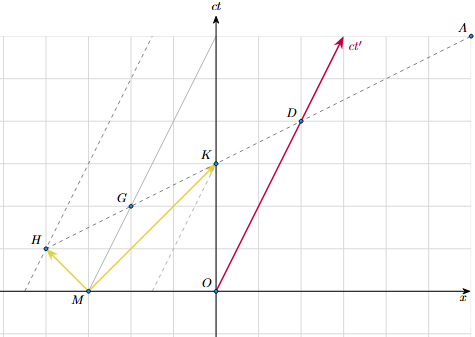
\includegraphics[width=0.5\textwidth]{Problem_1/Image/P1_8.png}
  \caption{}
  \label{P1_8}
  
\end{figure}
Tiếp tục khảo sát hệ quy chiếu của xe, ta thực hiện lại thí nghiệm tại thời điểm $t_{M}'$ ở $x_{G}'$, hai chớp sáng được phát ra đồng thời đi theo hai hướng và tới $H$ và $K$ cùng lúc . Thành thử $t_{H}'=t_{K}'$, và theo như kết quả ta vừa thu được ở \figref{P1_7}, $t_{H}'=t_{K}'=t_{G}'$. Lặp đi lặp lại như vậy với chân đường thế giới của các điểm đã được chứng minh là đồng thời ở trên, các điểm mới "lấp đầy" đường thẳng $AG$, hoặc nói cách khác, mọi điểm nằm trên đường thẳng $AG$ đều là các sự kiện có cùng thời điểm trong hệ quy chiếu của xe, tức đường thẳng $AG$ là một đường đồng thời gian. Ta cũng có thể hiểu điều này là tập hợp các điểm đồng thời trong hệ quy chiếu này vẫn lập thành một đường thẳng trong hệ quy chiếu khác. Với một đường thẳng bất kì trong một hệ quy chiếu nào đó, ta luôn có thể tìm thấy một hệ quy chiếu khác trong đó đường thẳng đó hoặc là đường đồng thời gian hoặc là đường đồng vị trí, nghĩa là một đường thẳng trong hệ quy chiếu này sẽ vẫn luôn là một đường thẳng trong hệ quy chiếu khác.\newline
Những điều trên dĩ nhiên cũng áp dụng cho đường đồng thời gian $t'=0$, đó chính là đường $EF$ mà trục $Ox'$ nằm trên đó. Nhận xét rằng trục $Ox'$ bây giờ đã không còn trùng hoặc song song với trục $Ox$ nữa.
\begin{figure}[H]
  \centering
  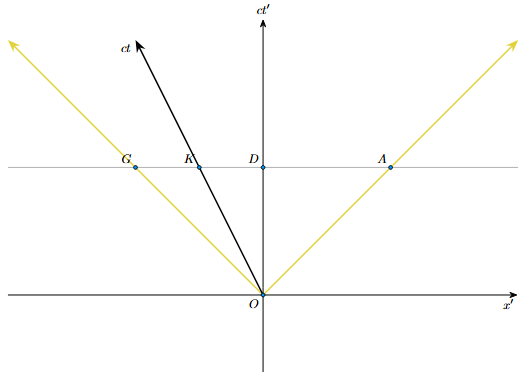
\includegraphics[width=0.6\textwidth]{Problem_1/Image/P1_9}
  \caption{Đường AG trong hệ quy chiếu của xe}
  \label{P1_9}
  
\end{figure}
\item  Dựa vào \figref{P1_7}, ta dễ dàng chứng minh được \begin{equation}
  \tan \angle{(ct)O(ct')}=\tan \angle{xOE}=\tan\angle {xOx'}=\frac{1}{2}.
\end{equation}
Nếu gọi góc này là $\theta$, bởi vì $O(ct')$ mô tả chuyển động của xe trong hệ quy chiếu của cây, do đó \begin{equation}
  \tan\theta=\frac{v}{c}=\beta.
\end{equation}
Nhận xét:
\begin{equation}
\begin{aligned}
  v \rightarrow 0:\quad & \beta \rightarrow 0 \text{, đường } Ox \text{ trùng với } Ox' \text{, phép biến đổi Galileo}\\
  v \rightarrow \pm c:\quad & \beta \rightarrow \pm 1 \text{, góc } \theta \text{ tiến đến } \pm 45^{\circ}\\
  \text{v>c} :\quad & \text{mâu thuẫn với nguyên lí nhân quả}
\end{aligned}
\end{equation}
Biểu diễn các đường đồng thời gian và vị trí của xe trong hệ quy chiếu của cây, ta vẽ được:
\begin{figure}[H]
  \centering
  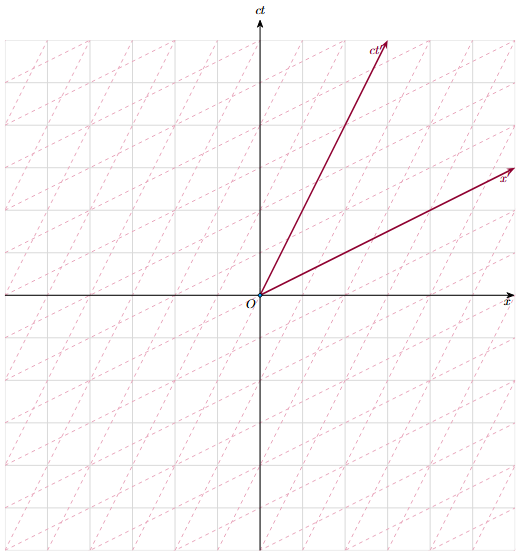
\includegraphics[width=0.5\textwidth]{Problem_1/Image/P1_10.png}
  \caption{Hệ lưới của xe trong hệ quy chiếu của cây}
  \label{P1_10}
\end{figure}
Thông qua các lập luận tương tự, ta xây dựng được hệ lưới của cây trong hệ quy chiếu của xe: $\angle (ct)O(ct')=\angle xOx'=\theta=\frac{v}{c}.$
\begin{figure}[H]
  \centering
  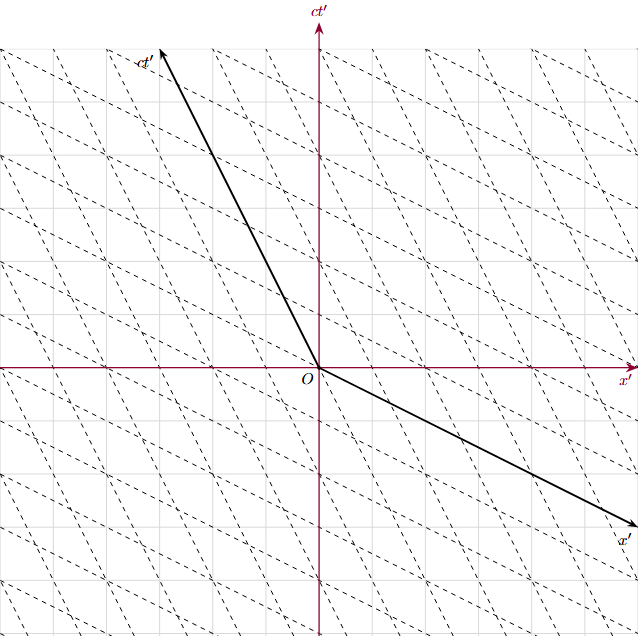
\includegraphics[width=0.55\textwidth]{Problem_1/Image/P1_12_2.png}
  \caption{Hệ lưới của cây được biểu diễn trong hệ quy chiếu của xe}
  \label{P1_12_2}
  
\end{figure}

\item
Khảo sát hệ quy chiếu của xe trong hệ quy chiếu của cây, ta xét điểm $M$ có toạ độ $(x,ct)$ trong hệ $xO(ct)$ và toạ độ $(x',ct')$ trong hệ $x'O(ct')$, để xác định vị trí và thời điểm của nó trong hệ quy chiếu của xe, ta chiếu $M$ song song với đường thế giới của xe tới trục $Ox'$ để thu được điểm $P$, chiếu $M$ song song với trục $Ox'$ tới đường thế giới của xe để được điểm $Q$. Giả sử $x'=1,ct'=1$, hình bình hành $OPMQ$ trở thành một hình thoi có độ dài là $k$ trong hệ quy chiếu của cây.  
\begin{figure}[H]
  \centering
  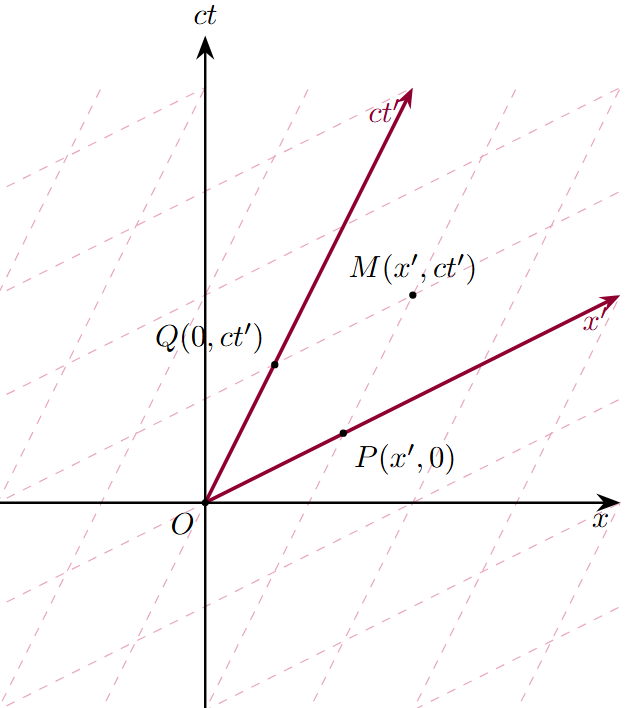
\includegraphics[width=0.6\textwidth]{Problem_1/Image/P1_11.png}
  \caption{}
  \label{P1_11}
\end{figure}
Biết rằng $\angle QOP=\frac{\pi}{2}-2\theta$,diện tích hình thoi $OPMQ$ đo trong hệ quy chiếu của cây là \begin{equation}
  S=k^2\sin^2 (\frac{\pi}{2}-2\theta).
\end{equation}
Song, trong hệ quy chiếu của xe, hình thoi này chỉ có diện tích $S'=1$, điều kiện bảo toàn diện tích nói rằng 
\begin{equation}
  k^2 \sin\!\left(\frac{\pi}{2} - 2\theta\right) = 1 \implies k^2 \cos 2\theta = 1
\end{equation}
Công thức nhân đôi:
\begin{equation}
\begin{aligned}
  \cos 2\theta &= \cos^2\theta - \sin^2\theta = 1-2\sin ^2\theta \\
  &= 1-2 \left[ \frac{1}{1+\frac{1}{\tan^2 \theta}}\right] 
  = \frac{1 - \tan^2\theta}{1 + \tan^2\theta} = \frac{1-\beta^2}{1+\beta^2} 
\end{aligned}
\end{equation}

Ta tính được k theo $\beta$:
\begin{equation}
  k = \frac{1}{\sqrt{\cos 2\theta}} = \sqrt{\frac{1+\beta^2}{1-\beta^2}}
\end{equation}
Kết quả này nói rằng nếu một "khoảng" có độ dài bằng $1$ trên giản đồ của xe thì khoảng đó sẽ có độ dài bằng $k$ trên giản đồ của cây. Điều ngược lại cũng đúng, nếu một khoảng có độ dài bằng $1$ trên giản đồ của cây thì sẽ có độ dài bằng $k$ trên giản đồ của xe: $k=k(v^2)=k((-v)^2).$ 

\item

\textbf{Co độ dài}

Không mất tính tổng quát, ta giả sử đầu bên trái của chiếc gậy nằm tại gốc tọa độ của hệ quy chiếu $S'$. Trên giản đồ Minkowski, hai điểm $A$ và $C$ biểu diễn hai đầu chiếc gậy tại cùng một thời điểm trong $S'$, nên $AC$ chính là độ dài riêng của chiếc gậy. Với $L_0=1$, độ dài hình học của đoạn $AC$ trên giản đồ là
\begin{equation}
AC=\sqrt{\frac{1+\beta^2}{1-\beta^2}}.
\end{equation}
Độ dài chiếc gậy trong hệ $S$ được xác định bởi khoảng cách giữa hai đầu tại cùng một thời điểm. Chọn $t=0$, khi đó độ dài đo được là đoạn $AB$. Gọi $\theta$ là góc nghiêng của các trục $x'$ và $ct'$, với
\begin{equation}
\tan\theta=\beta.
\end{equation}

\begin{figure}[htbp]
\centering
\begin{minipage}{0.48\textwidth}
  \centering
  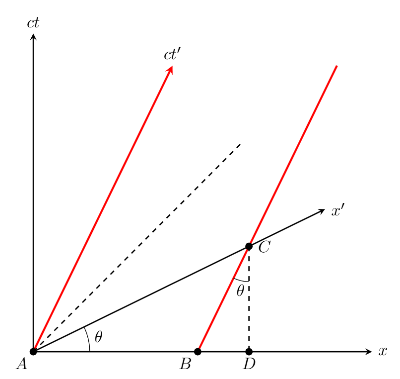
\includegraphics[width=0.8\linewidth]{Problem_1/Image/P1_12.png}
  \caption{}
  \label{P1_12}
\end{minipage}
\hfill
\begin{minipage}{0.48\textwidth}
  \centering
  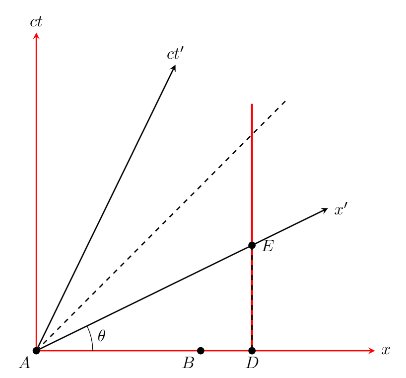
\includegraphics[width=0.8\linewidth]{Problem_1/Image/P1_13.png}
  \caption{}
  \label{P1_13}
\end{minipage}
\end{figure}

Từ hình học của giản đồ,
\begin{align}
AB
&=AC\cos\theta-AC\sin\theta\tan\theta \nonumber\\
&=AC\cos\theta(1-\tan^2\theta).
\end{align}
Thay $\tan\theta=\beta$ và giá trị của $AC$ vào, ta được
\begin{align}
AB
&=\sqrt{\frac{1+\beta^2}{1-\beta^2}}
\frac{1-\beta^2}{\sqrt{1+\beta^2}} \nonumber\\
&=\sqrt{1-\beta^2}.
\end{align}
Do đó,
\begin{equation}
L=L_0\sqrt{1-\beta^2}=L_0 \gamma,
\end{equation}

với $\gamma=\sqrt{1-\beta^2}$. 

\textbf{Giãn thời gian:}

Kết quả co độ dài cũng cho phép suy ra trực tiếp hiện tượng giãn thời gian. Thật vậy, xét một đồng hồ ánh sáng đứng yên trong hệ \(S'\), gồm hai gương cách nhau một khoảng \(L_0\). Trong hệ nghỉ của đồng hồ, thời gian để ánh sáng truyền từ gương này đến gương kia là

\begin{equation}
\Delta t'=\frac{L_0}{c}.
\end{equation}

Đối với người quan sát trong hệ \(S\), khoảng cách giữa hai gương bị co lại còn

\begin{equation}
L=L_0\sqrt{1-\beta^2}.
\end{equation}

Do vận tốc ánh sáng có cùng giá trị \(c\) trong mọi hệ quy chiếu quán tính, khoảng thời gian riêng và khoảng thời gian đo được trong \(S\) liên hệ với nhau bởi

\begin{equation}
\Delta t=\frac{\Delta t'}{\sqrt{1-\beta^2}}
=\gamma\Delta t'.
\end{equation}

\end{enumerate}

\emph{Lời bình:} \newline Phần hai của bài toán về tương đối tính Einstein được truyền cảm hứng bởi quyển sách \emph{An Illustrated Guide to Relativity by Tatsu Takeuchi}, xây dựng như một cách tiếp cận thuyết tương đối hẹp khác so với truyền thống. Đó là thay vì xây dựng phép biến đổi Lorentz từ hai tiên đề cơ bản, ta trực tiếp tiếp cận với giản đồ Minkowski, tức là bản chất hình học của lí thuyết với tinh thần phép chuyển hệ quy chiếu như là một phép biến đổi tuyển tính.\newline
Thuyết tương đối hẹp được xây dựng trên hai tiên đề là nguyên lí về sự tương đương của các hệ quy chiếu quán tính và nguyên lí về tính bất biến của tốc độ ánh sáng. Trong đó nguyên lí tương đương quan trọng hơn cả. Nguyên lí tương đương có hai nội dung chính: nếu một định luật vật lý đúng trong hệ quy chiếu (quán tính) này thì nó cũng đúng trong hệ quy chiếu khác, các hiện tượng quan sát được trong chúng phải là giống hệt; và không có sự khác biệt giữa các hệ quy chiếu (quán tính), điều này dẫn đến nhận định rằng mọi điểm trong không gian trống là tương đương vì mọi điểm đều có thể chọn làm một tập hợp tạo thành một hệ quy chiếu, như thế không gian là thuần nhất cũng như thời gian.\newline
Trong phần $(c)$, mục đích cốt lõi là xây dựng khái niệm ``đồng thời'' làm cơ sở cho các lập luận tiếp theo: chứng minh rằng một đường thẳng trong hệ quy chiếu này vẫn là một đường thẳng trong hệ quy chiếu kia, đồng thời xác định các đường đồng thời gian. Bản chất của chứng minh này là khẳng định các hàm $x(x',t')$, $t(x',t')$, $x'(x,t)$ và $t'(x,t)$ đều tuyến tính. Theo cách tiếp cận truyền thống, tính chất tuyến tính này thường được suy ra từ tính đồng nhất của không-thời gian, vốn là hệ quả của nguyên lí tương đối. Cụ thể, ta có thể lập luận rằng các vi phân của những hàm trên tại các điểm khác nhau là như nhau, từ đó dẫn đến việc các đạo hàm riêng theo từng biến là hằng số; tương đương với việc loại trừ sự xuất hiện của các số hạng phi tuyến, chẳng hạn các số hạng dạng $x\Delta x'$ hoặc các số hạng bậc hai. Trong lời giải này, thao tác toán học đó được thể hiện qua việc thực hiện các ``thí nghiệm'' tại một vài điểm rồi quy nạp cho cả đường thẳng, dựa trên giả thiết rằng mọi điểm trong không-thời gian đều có vai trò tương đương.\newline
Một điểm đáng chú ý khác đó là tính chất bảo toàn diện tích được mô tả trong ý $(d)$. Thực chất đó là một hệ quả trực tiếp và đẹp đẽ từ nguyên lí tương đương. Ta gọi $f$ là một ánh xạ mô tả tỉ lệ diện tích của hệ lưới sau và trước phép biến đổi\footnote{Một hàm như vậy có vai trò vô cùng quan trọng, nó được gọi là định thức của ma trận của phép biến đổi.} Lorentz (chính là phép đổi hệ quy chiếu cho một hệ lưới), đối với phép biến đổi từ hệ xe sang cây, ánh xạ này là hàm $f(v)$, ngược lại, với phép biến đổi từ cây sang xe, ta có hàm $f(-v)$. Bởi sự tương đương của hai hệ quy chiếu,  tất yếu rằng $\lvert f(v)\rvert=\lvert f(-v)\rvert$. Hơn nữa, giả dụ ta thực hiện liên tiếp một phép biến đổi từ hệ của xe sang cây rồi lại từ cây sang xe, hoặc ngược lại, ta phải thu được hệ ban đầu, nghĩa là $f(-v)\cdot f(v)=1$. Như vậy, $\lvert f(v)\rvert  =1$.  Song $f(v)$ không thể bằng $-1$ với mọi $v\in\mathbb{R}$, vì ta biết rằng $f(0)=1$: Ở giới hạn $v\to 0$, $f(v)$ chắc chắn liên tục, nên $f(v)\to 1$; tại lân cận $v=0$, $f(v)$ không thể nhảy vọt từ $1$ xuống $-1$, cứ thể trên toàn bộ miền giá trị của $v$, $f(v)$ chỉ có thể nhận giá trị bằng $1$. 

\vspace{0.5 cm}

\noindent \textbf{\large Phổ điểm}
\begin{center}
\renewcommand{\arraystretch}{1.5}
\begin{tabularx}{\textwidth}{|c|X|c|}
\hline
\textbf{Phần} & \textbf{Nội dung} & \textbf{Điểm thành phần} \\ \hline
a &Lập luận chỉ ra được phương trình chuyển động của các vật . & 0.25 \\ \cline{2-3} 
 & Vẽ được giản đồ không--thời gian. & 0.25 \\ \hline
b &Lập luận/vẽ ra các đường đồng vị trí, đồng thời gian. & 0.25 \\ \cline{2-3} 
 &Chỉ ra cách xác định một điểm tọa độ (x,t) khi biết tọa độ (x',t') của nó qua hình vẽ. & 0.25 \\ \hline
c &Vẽ được các đường thế giới của photon và các vật trong 2 hệ quy chiếu. & 0.5 \\ \cline{2-3} 
 &Lập luận được các sự kiện không còn đồng thời. & 0.5 \\ \hline
d &Biểu diễn lại các đường đồng thời gian và đồng vị trí. & 0.25 \\ \cline{2-3} 
 &Chỉ ra $\tan \theta = v/c$ và các giới hạn. & 0.25 \\ \hline
e &Tính được diện tích ô đơn vị của giản đồ. & 0.25 \\ \cline{2-3} 
 & Tính được k. & 0.25 \\ \hline
f &Xây dựng được mô hình co độ dài và giãn thời gian. & 0.25 \\ \cline{2-3} 
 &Tìm được hệ số $\gamma$. & 0.25 \\ \cline{2-3} 
& Tìm được hệ thức liên hệ của các ảnh hưởng & 0.5 \\ \hline
\multicolumn{2}{|r|}{\textbf{Tổng điểm}} & \textbf{4.0} \\ \hline
\end{tabularx}
\end{center}